\section{Working of YouTube: A 1000 Feet View}
\label{sec:overview}

\begin{figure}[!t]
	\centering
	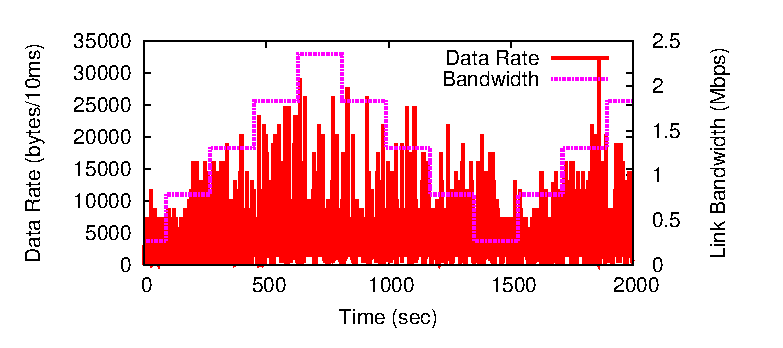
\includegraphics[scale=0.85]{img/burst.eps}
	\caption{Packet length distribution}
	\label{fig:packet}
\end{figure}

\begin{figure}[!t]
	\centering
	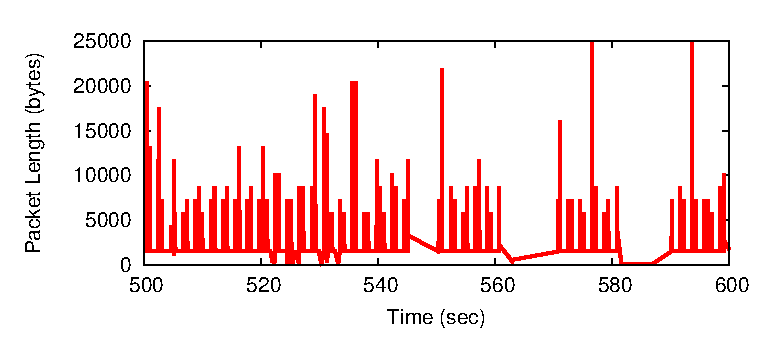
\includegraphics[scale=0.85]{img/burst_scale.eps}
	\caption{Packet bursts with respect to time}
	\label{fig:burst}
\end{figure}

\begin{figure}[!t]
	\centering
	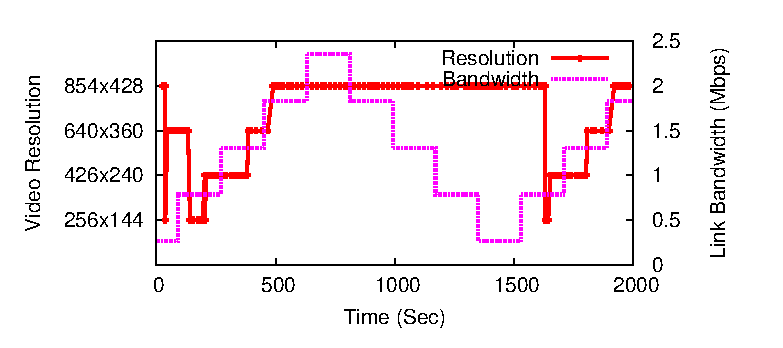
\includegraphics[scale=0.85]{img/bw_reso.eps}
	\caption{Video resolution vs link bandwidth}
	\label{fig:reso}
\end{figure}



% What led to the study - our observations from traffic analysis\\
% An introduction to the DASH protocol\\
% An overview of how Youtube DASH works

To understand the behavior of YouTube under different traffic conditions, we first execute a few motivational experiments to figure out how the change in link bandwidth affects video streaming in YouTube. 
%\noteng{Would be good if all the figures are made in one block}

\subsection{Experimental Setup}
In the preliminary experiment, we play a YouTube video (video title: {\em ``The Division Walkthrough Gameplay Part 1 -- The Virus (PS4 Xbox One)''}, video ID: {\em b80ShWk\_Aro}, URL: \url{https://www.youtube.com/watch?v=b80ShWk_Aro}, video duration: $34$ minutes $22$ seconds) by varying the link bandwidth using a dynamic throttling mechanism as follows. We use the Unix library \texttt{NetFilterQueue}~\cite{nfqueue} to implement link throttling; it is a user-space library that provides an API to handle packets, which have been queued by the kernel packet filter, as per user requirement. Based on this library, we develop a traffic shaper to control link bandwidth. However, we continuously monitor and ensure that the backbone network has sufficient bandwidth so that the overall link bandwidth is controlled only by the throttling procedure. 

During the video playback, we capture video data packets using the Unix tool \texttt{tcpdump}. From these packet traces, we extract the amount of video data transferred from the YouTube server to the YouTube client, with respect to time. Further, during video playback, we note down the resolution in which the video is rendered, with respect to time. 

\subsection{Observations and Analysis}

Fig.~\ref{fig:packet} and Fig.~\ref{fig:burst} show the sequence of packets received from YouTube server to YouTube client with respect to time and changing link bandwidth, while Fig.~\ref{fig:reso} indicates the video playback resolution with respect to time. In both the graphs, we show the change in link bandwidth (through the throttling mechanism) with respect to time, using the right hand side Y-axis. From Fig.~\ref{fig:packet}, we can clearly observe that packet length increases with increase in link bandwidth, and drops when link bandwidth is decreased. Fig.~\ref{fig:burst} shows the sequence of packets received by scaling up the time axis, and this figure indicates that in YouTube, packets are indeed transferred in bursts. A group of packets are transferred and buffered at the YouTube client, and then there is a silent zone when no packet is transferred. From these two figures it is clear that YouTube dynamically changes content length in data packets based on link bandwidth. It transfers content in data bursts, and reduces (increases) the content length when link bandwidth is low (high). 

Next, we observe the impact of link bandwidth on video playback/rendering resolution as plotted in Fig.~\ref{fig:reso}. The figure indicates that YouTube increases playback resolution as the link bandwidth improves. It keep on rendering the video at high resolution till it has high resolution video data in its buffer, and if the link bandwidth drops by that time, it starts buffering as well as rendering video at lower resolution. In the figure, we can see that YouTube keeps on playing the video at high resolution till $1600$ seconds, as it has already received the data for high resolution, and as the link bandwidth drops by that time, the playback video resolution also drops for the new data that it receives. However, after that as the link bandwidth increases, YouTube progressively improves the playback video resolution by downloading higher resolution video content.

\subsection{Open Questions: What is Interesting in YouTube Video Streaming?}

From the above experiment, we observe that based on the change in link bandwidth, YouTube not only changes the video resolution, but also changes the content length of the data packets. Therefore it gives us an indication that YouTube uses a progressive download mechanism, where both the content type and content length get changed based on the link condition. These initial observations regarding YouTube adaptive video streaming raise few interesting questions regarding how YouTube implements the recommendations of DASH specifications. 
\begin{enumerate}
	\item {\em What is the feedback mechanism from YouTube client to YouTube server}, based on which YouTube adaptively changes both the video resolution and the content length of data packets?  Does YouTube directly observe the link quality or use some other derived parameters that give an indication of future link quality? 
	\item Fig.~\ref{fig:reso} demonstrates an interesting property of YouTube video streaming -- when the link quality improves, YouTube uses a progressive mechanism for step-by-step improvement in video resolution. However, when link quality drops, video quality directly drops to the lowest resolution in a conservative approach. Then again, YouTube applies progressive improvements of video resolution as the link quality keeps on improving. Apparently, {\em this mechanism looks analogous to TCP's progressive congestion control mechanism}. The question here is: {\em How does YouTube decide which parameter to tune -- video quality or content length per data packet, and whether there are some relationships between the tuning of these two parameters and the link bandwidth?}.  
\end{enumerate}

With these motivations to understand the internals of YouTube adaptive video streaming mechanism and to make it one of the benchmarks for comparison with other open-source DASH based adaptive video streaming protocol implementations, we apply a reverse engineering methodology to explore how YouTube works in practice. In the next section, we provide the details of the experimental setup used in our reverse engineering approach and analyze the findings.


\begin{comment}
\subsection{Background and Preliminaries}
\label{chap03s1:sec:background}
In this section, we provide the reader with a detailed background on YouTube's video streaming strategy.
{\bf Evolution of YouTube's playback mechanism:} Since its inception in $2005$, viewing videos on YouTube required the Adobe Flash plug-in to be installed on the user's browser\footnote{\url{http://news.bbc.co.uk/2/hi/8287239.stm}}.
In an attempt to reduce third party dependency, and to take advantage of the HTML5 standard which allowed embedded multimedia, YouTube launched an experimental version of the site in January $2010$.
The service, which encompassed only a section of available videos, was extended to users who opted-in for the trial\footnote{\url{https://www.youtube.com/html5}} and were on a browser which supported HTML5 video using WebM or H.264 formats.
YouTube experimented with {\it Dynamic Adaptive Streaming over HTTP (DASH)} around 2013\footnote{\url{https://www.youtube.com/watch?v=UklDSMG9ffU}} to elevate quality of experience of viewers, before adopting it as the default playback mechanism on January 27, 2015\footnote{\url{https://arstechnica.com/gadgets/2015/01/youtube-declares-html5-video-ready-for}\\\url{-primetime-makes-it-default/}}.

\begin{figure}[!t]
 \centering
 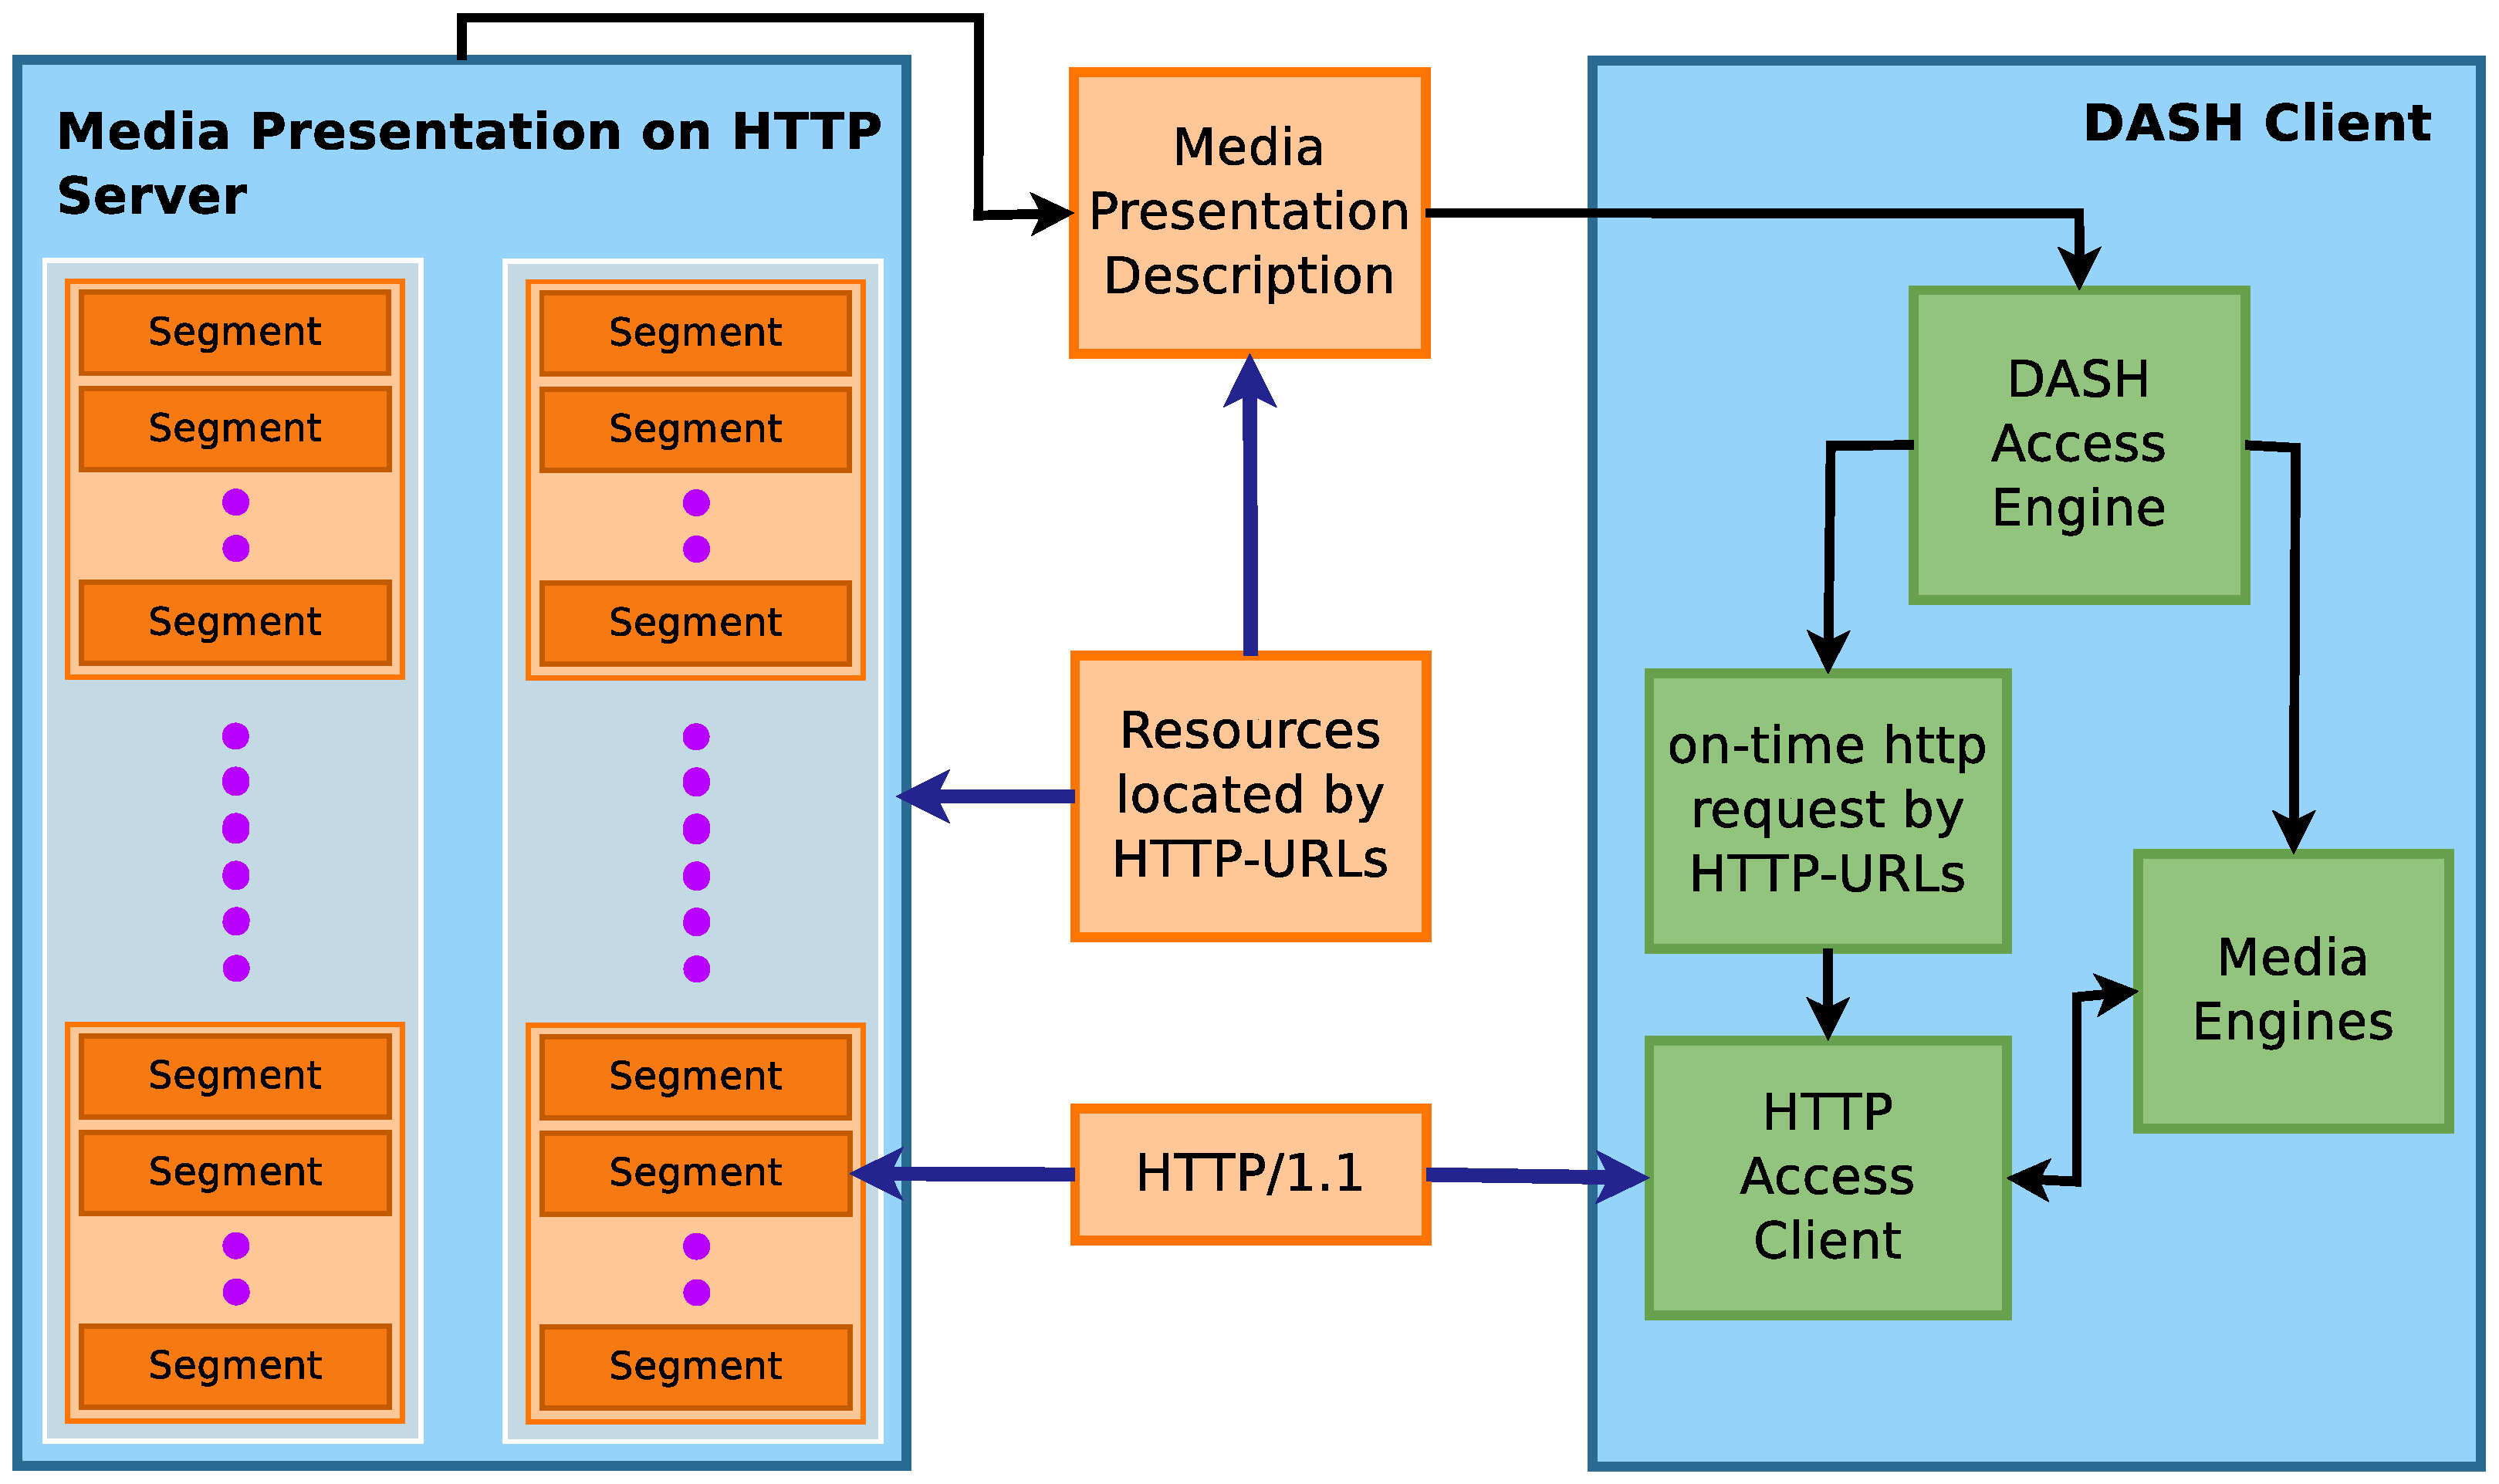
\includegraphics[width=0.7\linewidth]{img/dash-arch}
 \caption{\small{DASH Architecture -- On the left side, the server-side media storage is shown, where content is divided into small segments of alternative bit-rates. On the right side, the DASH client architecture is shown; the {\it DASH Access Engine} monitors network bandwidth at the client and accordingly decides which segment to request from the server. (Image Source: https://www.w3.org/2011/09/webtv/slides/W3C-Workshop.pdf)}}
 \label{fig:chap03s1:dash}
\end{figure}
{\bf DASH specifications:} Dynamic Adaptive Streaming over HTTP (DASH), also referred to as MPEG-DASH, is an adaptive bit-rate solution for video streaming, which enables client-operated video delivery over HTTP.
DASH is implemented by breaking down the video content into small segments, each worth a short duration of playback time.
For every segment of playback time, alternative versions at various bit-rates are available at the server.
The client typically requests for the highest quality segment possible under current network conditions, such that it is received (downloaded) in time for playback, without causing stalling or re-buffering. 
However, DASH is not a protocol -- it only specifies an architecture (Fig.~\ref{fig:chap03s1:dash}) to enable adaptive video streaming over HTTP.
Every video streaming service (e.g., YouTube, Netflix, etc.) is free to define its own implementation of the DASH modules.
In this work, our aim is to study in depth YouTube's implementation of the {\it DASH Access Engine} module (as seen in Fig.~\ref{fig:chap03s1:dash}).

{\bf Encoding technique:} YouTube uses the VP9 codec\footnote{\url{https://youtube-eng.googleblog.com/2015/04/vp9-faster-better-buffer-free-youtube.html}}, which is a free video codec developed by Google to serve YouTube video.
The codec specifies that video files encoded using it shall consist of two types of frames -- (1) key-frame, and (2) intra-frame; key-frames contain complete frame information, while every subsequent intra-frame contains incremental information relative to the last seen key-frame.
Such specifications mandate that a VP9 decoder can start decoding only at key-frames, an observation we utilize to model data consumption more accurately in \S\ref{chap03s1:sec:model}.

{\bf Related Works:} Existing studies on YouTube streaming and quality of experience (QoE) can be grouped into two broad classes.
The first class of works explore traffic patterns and video QoE properties of YouTube~\cite{gill2007youtube,krishnappa2013dashing,wamser2016modeling,wamser2015poster,6757893ieeeexp,7129790ieeeexp}.
These papers mostly study YouTube behavior at the periphery, which although provides a summary of performance metrics, but fails to say much about the internals of YouTube's video streaming protocol.
The second class of studies, however, explore adaptive streaming characteristics of YouTube.
In \cite{finamore2011youtube}, the authors investigate YouTube's data delivery system from the end user view, and illustrate evidence of massive wastage of downloaded data, since viewers often do not watch entire videos -- the study, however, was performed at a time when YouTube used progressive download as the streaming mechanism, and is therefore stale.
\cite{krishnappa2013dashing} is probably the first work to evaluate YouTube's performance since its adoption of adaptive streaming -- the authors claim that YouTube gains $83\%$-$95\%$ in terms of bandwidth by switching from progressive download to DASH.
Some recent works~\cite{sieber2015cost,seufert2015youtube,sieber2016sacrificing} study YouTube's DASH behavior to analyze the trade-off between quality and data wastage -- however, as already pointed out in~\S\ref{chap03s1:sec:introduction}, their approximations lead to gross overestimation. they perform controlled experiments by varying the underlying link bandwidth, and compute wastage.

\end{comment}
